\IEEEraisesectionheading{\section{Introduction}\label{sec:introduction}}
% Computer Society journal (but not conference!) papers do something unusual
% with the very first section heading (almost always called "Introduction").
% They place it ABOVE the main text! IEEEtran.cls does not automatically do
% this for you, but you can achieve this effect with the provided
% \IEEEraisesectionheading{} command. Note the need to keep any \label that
% is to refer to the section immediately after \section in the above as
% \IEEEraisesectionheading puts \section within a raised box.




% The very first letter is a 2 line initial drop letter followed
% by the rest of the first word in caps (small caps for compsoc).
% 
% form to use if the first word consists of a single letter:
% \IEEEPARstart{A}{demo} file is ....
% 
% form to use if you need the single drop letter followed by
% normal text (unknown if ever used by the IEEE):
% \IEEEPARstart{A}{}demo file is ....
% 
% Some journals put the first two words in caps:
% \IEEEPARstart{T}{his demo} file is ....
% 
% Here we have the typical use of a "T" for an initial drop letter
% and "HIS" in caps to complete the first word.
%file is intended to serve as a ``starter file'' for IEEE Computer Society journal papers produced under \LaTeX\ using IEEEtran.cls version 1.8b and later.
% You must have at least 2 lines in the paragraph with the drop letter
% (should never be an issue)
 
\IEEEPARstart{H}{igh-}throughput sequencing~(HTS) is the standard for deep and detailed studies in many areas such as population genomics and precision medicine. As the vision of predictive, preventive, personalized, and participatory~(P4) medicine~\cite{flores2013p4} rapidly becomes more prevalent, sequencing technologies stand out to provide vital information as a base for further investigation. Sequencing data generated by HTS constitutes a reliable source for biological research pipelines. 

%\todo{2.HTS produces Big Genomics Data} 
As a result of massively parallel sequencing, a tremendous amount of data can now be generated in a single run~\cite{xin2013accelerating, arram2017leveraging}, making genomics one of the largest sources of big data today and in the future~\cite{stephens2015big}. On the other hand, the enormous data creates a computational challenge for analysis regarding both runtime and memory footprint, emphasizing the importance of developing efficient methods for quickly and efficiently analyzing genomic data.

% \todo{3.Why is it important to speed up the process}
The first main step in genome analysis is either \textit{de novo assembly}~\cite{chaisson2015genetic} or \textit{read mapping}, depending on the goal of the study. For read mapping, the reference genome of the subject species stands as a template~\cite{ruffalo2011comparative}, and newly sequenced fragments of a genome are compared to it to understand the genetic material of the individual sample. Read mapping consists of two main stages: \textit{seeding} and \textit{verification} (i.e., sequence or read alignment). In the seeding stage, the potential locations of reads on the reference genome are found based on the string similarity between the reads and corresponding reference segments~\cite{alser2021technology}. Reads generally have more than one possible seed location on the reference genome due to genomic repeats~\cite{Treangen2012} and the seeding strategy.

One of the most popular approaches to finding the possible locations that fit the read on the reference genome is the \textit{seed-and-extend} strategy~\cite{altschul1990basic}. This approach is rooted in the idea that two similar sequences share exactly or approximately matching substrings~(i.e., seeds, kmers)~\cite{ahmed2016comparison}. Consequently, once the matching locations of the shorter substrings, which are extracted from the read, are found on the reference genome, the seeds can then be \textit{extended} to form the candidate reference segment (Figure \ref{fig:seed-n-extend}). Since kmers are shorter than reads, the seeds may map to many locations, eventually creating multiple mapping locations for a single read.
\vspace{-2mm}

%%%%%%%%%%%%%%%%%%%%%%%%%%%%%%%%%%%%%%%%%%%%%%%%%
% Fig: Seed-and-Extend 
\begin{figure}[!htbp]
\hspace{1cm}
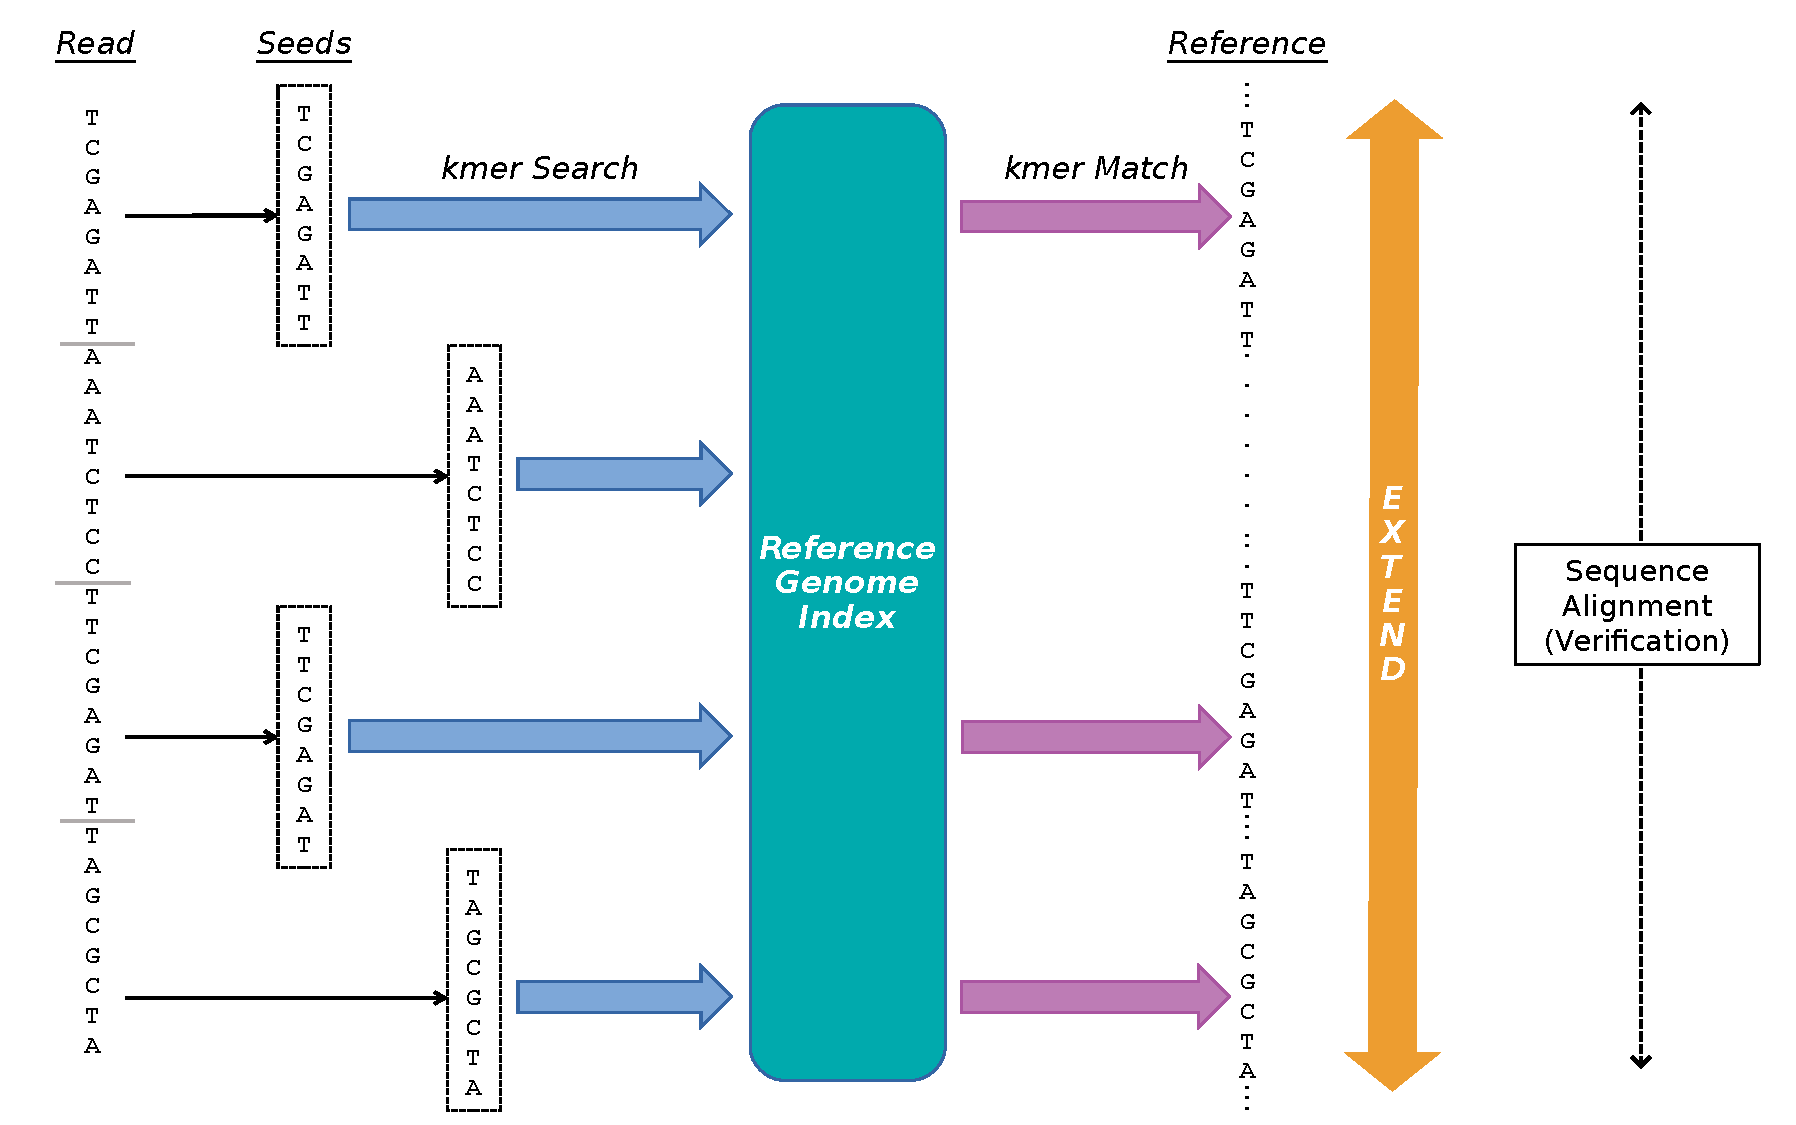
\includegraphics[width=0.4\textwidth, height=5cm]{figures/seed_n_extend4.pdf}
\caption{High-level view of seed-and-extend paradigm.}
\label{fig:seed-n-extend}
\end{figure}
%%%%%%%%%%%%%%%%%%%%%%%%%%%%%%%%%%%%%%%%%%%%%%%%%%%

%\todo{4.Approximate String Matching Problem}
The presence of possible sequencing errors~\cite{shendure2008next} and base mutations restrict the use of an exact string matching algorithm, such as Hamming Distance~\cite{hamming1950error} or KMP~\cite{knuth1977fast}, for mapping the reads to the reference genome. Therefore, verifying the actual locations requires \textit{approximate string matching} techniques on strings with a predefined error threshold~\cite{alser2020accelerating}. Once all of the candidate locations are found by seeding, the read's most accurate location on the genome among all of its candidates is decided upon verification. Traditional practices generally lean towards using dynamic programming algorithms~\cite{alser2021technology} such as Needleman-Wunsch~\cite{needleman1970general}, Smith-Waterman~\cite{Smith1981}, and Levenstein Distance~\cite{levenshtein1966binary} to confirm that the distance between extended sequence segment from reference and the read is within the limits of an error threshold. However, dynamic programming solutions are computationally expensive with quadratic time and space requirements~(i.e., O($n^2$) for a sequence length of \textit{n}). Since seeding produces many candidate reference locations because of genomic repeats, performing alignment for every pair becomes a bottleneck. 

%\todo{4.necessity for prealignment filtering}
Due to the compute-intensive nature of dynamic programming solutions, the verification step creates a bottleneck for the entire read mapping procedure. Therefore, efficient amendments targeting this stage are expected to improve the entire process~\cite{alser2020accelerating}. The conspicuous approaches to address this problem would be either improving the algorithms in terms of time and space complexities~\cite{myers1999fast, zhang2000greedy} or reducing the workload on verification so that the pipeline visits verification as rarely as possible. In this work, our goal is to significantly reduce the execution time of read alignment by adopting the second approach and eliminating the candidate locations that exceed a predefined error threshold with fast and accurate pre-alignment filtering.
 
 %\todo{5.GateKeeper-GPU}
We propose GateKeeper-GPU, a fast and accurate general-purpose graphics processing unit~(GPGPU) pre-alignment filter for short read mapping to be performed before verification. GateKeeper-GPU is established on two key ideas:~1)~improving the filtering accuracy of GateKeeper~\cite{Alser2017}, which is a computationally lightweight pre-alignment filter, and~2)~employing massive parallelism provided by a large number of modern GPU threads for concurrent and quick examination of numerous sequence pairs. 
 
GateKeeper's original codebase is developed for field programmable gate array~(FPGA) devices. We opt for implementing it on general-purpose GPUs with the CUDA framework for several reasons. First, GPU has a large number of specialized cores~(i.e., 3584 CUDA cores in NVIDIA Geforce GTX 1080 Ti~\cite{cudacores}) that have smaller caches when compared to CPU cores; thus, its cores require lower frequency. This makes GPU a powerful candidate for processing the work for which the throughput is crucial~\cite{mittal2015survey}. Since pre-alignment filtering requires high throughput to complete as many comparisons as possible before verification, GPU is well-suited for this work. 
Second, although FPGA can provide more adjustable hardware designs, GPU is easier to install and use than FPGA because it does not require an in-depth understanding of the underlying hardware. Once installed, GPU can be used in a wide range of applications without extra configuration effort.
Third, GPU implementation is fully configurable at compile-time and runtime, such that the input parameters~(e.g., error threshold) can be changed without any alteration in the implementation.
On the other hand, the FPGA codebase requires changing the architecture design for each different parameter value. Therefore, we aim to provide easy usage and support for various platforms by implementing GateKeeper-GPU.

%\todo{Our contributions}
This paper makes the following \textbf{contributions}:
\begin{itemize}
\item We introduce GateKeeper-GPU, a new fast and accurate GPU-based pre-alignment filter with an improved GateKeeper algorithm and CUDA framework to facilitate a wider range of platform usage with GPGPUs.
\item We integrate GateKeeper-GPU with mrFAST to show its performance gain in a short read mapper with full workflow. This will hopefully serve as an example to embed GateKeeper-GPU to any short read mapping tool easily. 
\item We provide comprehensive analyses about the accuracy, filtering throughput, power, and resource utilization using two different device setups. We show that GateKeeper-GPU can accelerate the verification stage by up to $2.9\times$ and provide up to $1.4\times$ speedup for overall read mapping procedure when integrated with mrFAST \cite{alkan2009personalized}, in opposition to having no pre-alignment filter. Compared to the original GateKeeper~\cite{Alser2017}, GateKeeper-GPU produces up to $52\times$ less false accepts in candidate mappings.
\end{itemize}